\section{Requisitos específicos}
\subsection{Interfaces externos}
\subsection{Requisitos funcionales}
\subsubsection{Gestión de usuarios}%USUARIOS
\paragraph{Alta cliente}
El usuario introduce su nombre usuario y contraseñas deseados en el sistema. Tras introducir los datos el sistema determina si ya existe dicho usuario. Si el nombre de usuario ya existe en la \gls{bd}, se informa de que dicho nombre no es valido. Si el nombre de usuario no se encuentra en la \gls{bd}, se procede a guardar los datos en la \gls{bd} y se informará al usuario del éxito de la operación.
\begin{figure}[H]
    \centering
    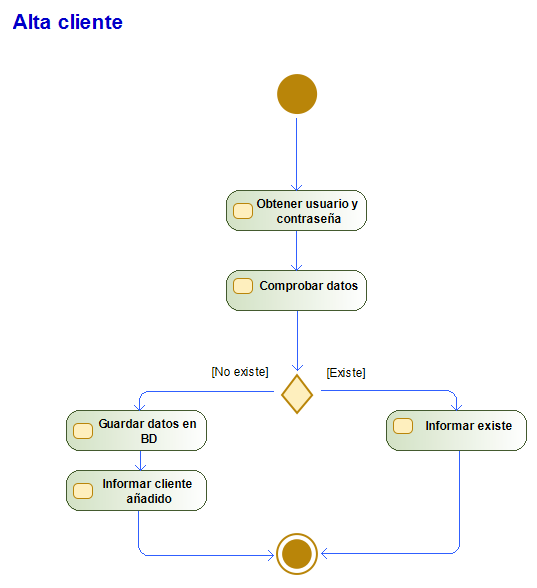
\includegraphics[width=0.8\textwidth]{Use_Cases/alta_cliente.png}
\end{figure}
\paragraph{Baja cliente}
El usuario solicita al sistema su baja, el administrador comprueba en la \gls{bd} si el usuario existe. En caso de ser encontrado, se borrarán sus datos de la \gls{bd}. En caso contrario, se informará al usuario de que no ha sido encontrado en la \gls{bd}
\begin{figure}[H]
    \centering
    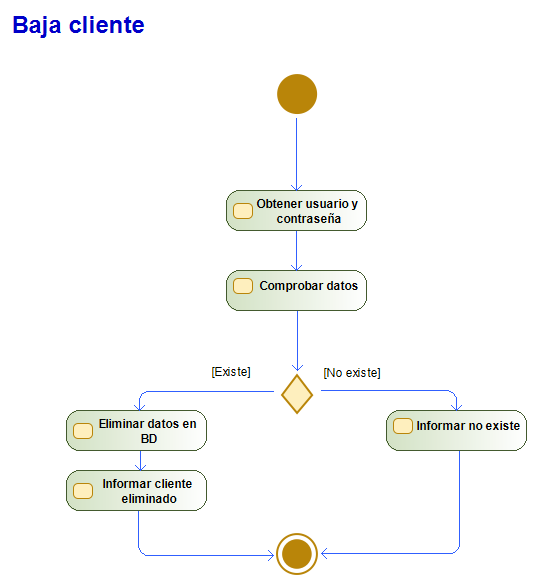
\includegraphics[width=0.8\textwidth]{Use_Cases/baja_cliente.png}
\end{figure}
\paragraph{Añadir Administrador}
Se solicita el usuario sus datos, un nombre de usuario y una contraseña. Si los datos coinciden se procede a buscar los datos del administrador en la \gls{bd}. En caso contrario, se informa de que los datos aportados no son válidos. Al buscar en la \gls{bd}, si el usuario no existe, se creará y se le darán permisos de administrador. En caso de ya existir, se avisará de ello.
\begin{figure}[H]
    \centering
    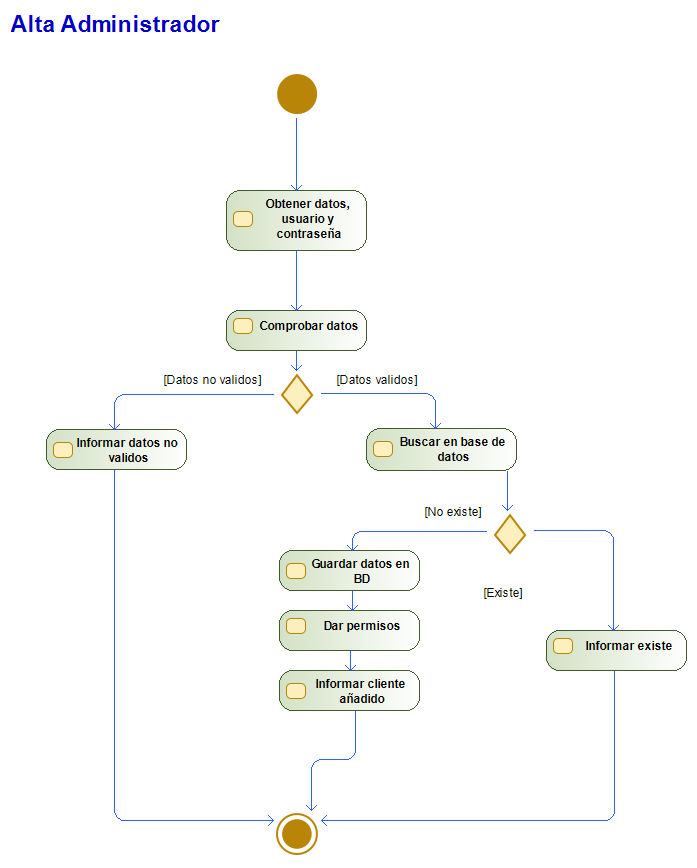
\includegraphics[width=0.8\textwidth]{Use_Cases/alta_admin.png}
\end{figure}
\paragraph{Baja administrador}
Se obtienen los datos del administrador y se buscan en la \gls{bd}. Si se encuentran se le quitarán permisos y se borrará el usuario, al terminar se informará del éxito de la operación. Por el contrario, si no se encuentra el usuario, se informa  de que se ha producido un error.
\begin{figure}[H]
    \centering
    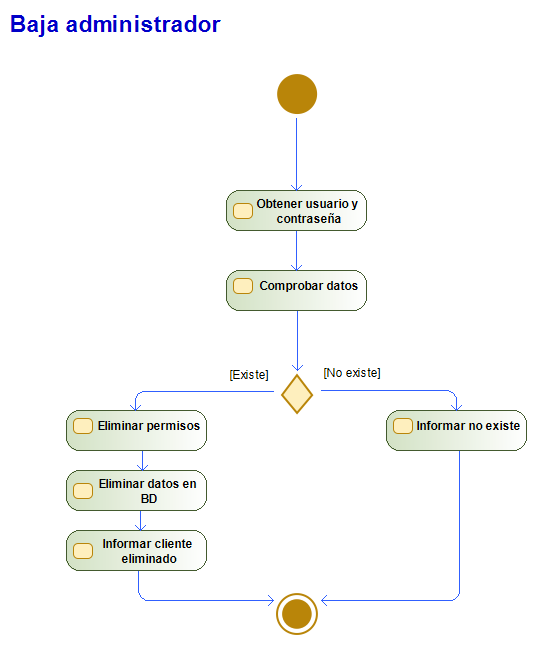
\includegraphics[width=0.8\textwidth]{Use_Cases/baja_admin.png}
\end{figure}
\paragraph{Alta empleado}
\paragraph{Baja empleado}
\paragraph{Sancionar cliente}
\paragraph{Cambiar nombre}
\paragraph{Cambiar contraseña}
\paragraph{Login}
\paragraph{Logout}
\subsection{Gestión de inventario}
\paragraph{Añadir producto}
\paragraph{Buscar producto}
\paragraph{Actualizar stock}
\paragraph{Quitar producto}
\paragraph{Aplicar descuento}
\paragraph{Informar de desperfecto}
\subsection{Gestión de pedidos}
\paragraph{Añadir promoción}
\paragraph{Quitar promoción}
\paragraph{Compras}
\paragraph{Devolución de pedido}
\paragraph{Reservar producto}
\subsection{Requisitos de rendimiento}
\subsection{Requisitos sobre la persistencia de datos}
\subsection{Restricciones de diseño}
\subsection{Atributos del sistema software}
